\section{Research Runtime and Mission Lifecycle}
\label{sec:runtime}

\begin{designbox}
Run one mission at a time, back to back, for days --- surviving restarts,
upgrades, and provider outages --- without ever re-deciding a committed campaign
or killing a mission mid-flight. The unit of scheduling is a mission; the unit of
durability is the mission boundary.
\end{designbox}

The research runtime is the 7$\times$24 loop that turns a durable objective into a
stream of missions. Figure~\ref{fig:lifecycle} shows the lifecycle and its
recovery edges. This section describes the states, the process model, and the
restart/resume semantics that make a long campaign durable.

\begin{figure}[ht]
\centering
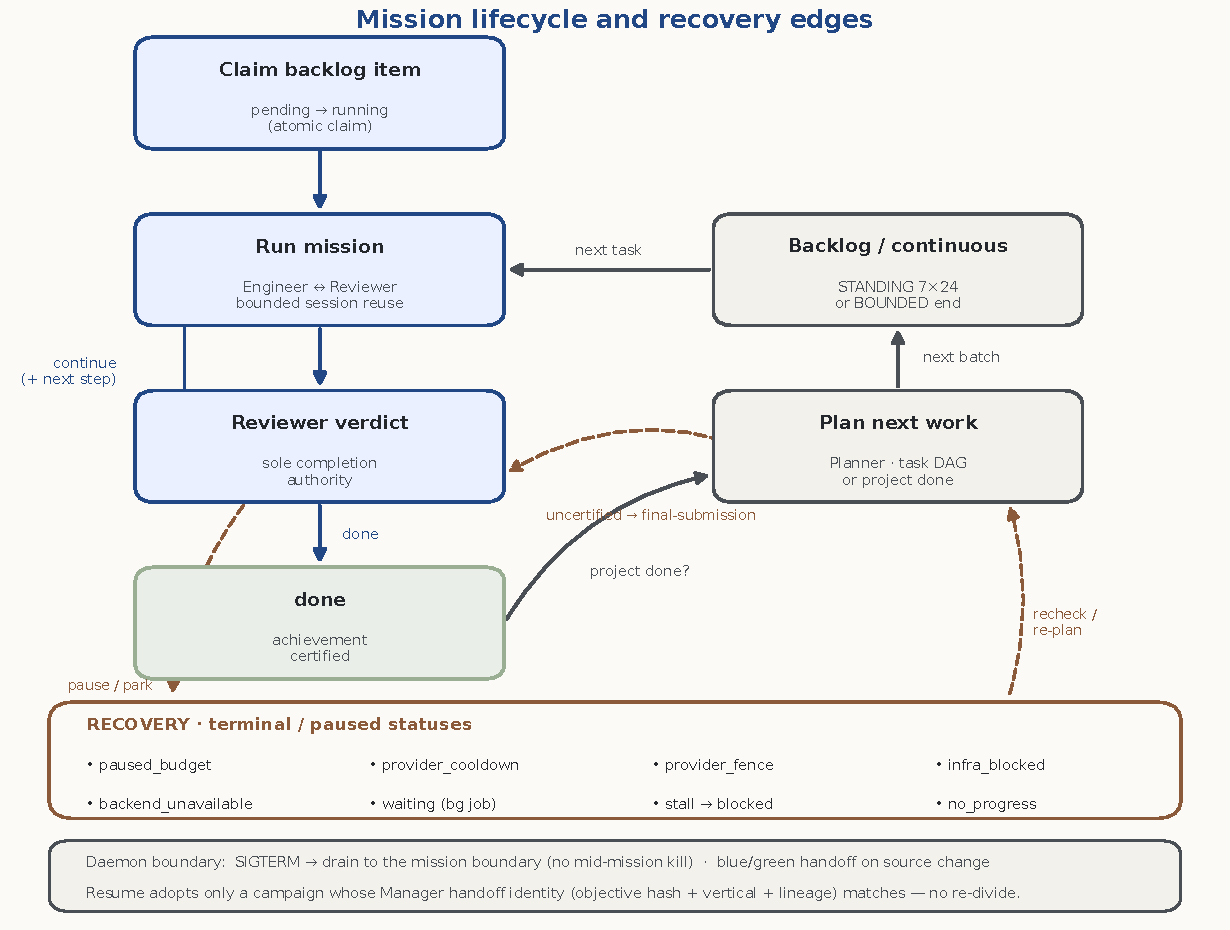
\includegraphics[width=0.9\textwidth]{figures/mission_lifecycle.pdf}
\caption{Mission lifecycle and recovery edges. The primary spine (indigo) claims
a backlog item, runs an Engineer$\leftrightarrow$Reviewer mission, and acts on the
Reviewer verdict; the plan-next loop (grey) refills the backlog; recovery edges
(terracotta) route paused and blocked missions to first-class statuses and back.
The daemon boundary governs draining, handoff, and identity-checked resume.}
\label{fig:lifecycle}
\end{figure}

\subsection{From objective to missions}

An objective enters through the Manager, which \emph{divides} it: it selects one
vertical and commits it durably. From that point the scheduler \emph{trusts} the
persisted vertical and never re-classifies the task --- a single division decision,
not a per-round guess.\footnote{\srcpath{manager/\_core.py}; the scheduler reads
the committed vertical rather than re-running the Manager.} A task's
\emph{lifetime} is likewise an explicit, Manager-decided property: most team tasks
default to \code{STANDING} (run 7$\times$24) and are persisted atomically to
\code{continuous.json}; a task with a natural one-shot endpoint is
\code{BOUNDED}. An operator may force \code{BOUNDED} at daemon start with
\code{--bounded}.

The Manager also owns pipeline-stage progression. A vertical supplies an ordered
stage template (\code{STAGE\_ORDER}); the Manager advances \code{current\_stage}
through it via a stage decision whose \code{action} is one of \code{advance},
\code{hold}, \code{rollback}, or \code{complete}, with a \code{source} field that
records \emph{why} (a model decision, or one of several fail-safe holds). The
Planner, Engineer, and Reviewer may advise a stage change but never write it
(Section~\ref{sec:roles}).

\subsection{The mission scheduler}

The \code{LifeSupervisor} runs a synchronous outer loop: it claims the next
backlog item, injects a non-authoritative recency memory preamble without
polluting the raw objective, runs the mission through the execution plane,
accounts the cost against budget gates, writes a journal entry, and --- when the
backlog empties in continuous mode --- invokes the Planner for the next batch. The
backlog claim (\code{pending}$\rightarrow$\code{running}) is atomic, so two
workers can never take the same item; orphaned \code{running} items from a prior
crash are reaped on startup.\footnote{\srcpath{life/supervisor/\_core.py};
atomic \code{Backlog.claim\_next} and startup orphan reaping.} The scheduler is
deliberately synchronous --- one mission at a time --- which is what makes the
mission boundary a clean, well-defined point for stopping, upgrading, and
resuming.

Every mission ends in a first-class terminal or paused status, never an
unbounded spin. Terminal outcomes include \code{done}, \code{blocked},
\code{max\_rounds}, \code{no\_progress}, and \code{error}; paused outcomes
include \code{paused\_budget}, \code{paused\_provider\_cooldown},
\code{paused\_provider\_fence}, and \code{infra\_blocked} (the full taxonomy is in
Appendix~\ref{app:status}). A paused mission is not a failure: it records that
the campaign is correctly waiting on an external condition and should be rechecked
later.

\subsection{Process model: the daemon}

For unattended operation the runtime runs as a detached daemon worker
(\srcpath{daemon/life\_worker.py}, roughly 1{,}800 lines) wrapping the
supervisor. Two properties make it safe to run continuously.

\begin{description}[leftmargin=1.4em, style=nextline]
  \item[Drain to the mission boundary.] On \code{SIGTERM} or \code{SIGINT} the
    worker stops cleanly at the next mission-tick boundary rather than
    interrupting a live mission, so an in-progress evaluation or a result being
    recorded is never severed.
  \item[Two-layer concurrency guard.] A run is protected by both the atomic
    backlog claim and a per-project \code{daemon.pid} lock
    (\srcpath{core/daemon\_lock.py}), so a second daemon cannot drive the same
    project. Continuous-mode configuration is coordinated per project through
    \code{continuous.json}, which the worker hot-reloads.
\end{description}

\subsection{Upgrades: blue/green handoff and identity-checked resume}

A 7$\times$24 system must be upgradable without losing a campaign. Argus handles a
source change with a \textbf{blue/green self-handoff}: the worker detects a change
in its own source signature, spawns a candidate child process under an
environment-driven handoff protocol with bounded generation count and a minimum
inter-handoff interval, and hands the campaign over at a clean boundary
(\srcpath{daemon/handoff.py}). The Manager-to-daemon handoff \emph{identity}
(objective hash, vertical, lineage generation) is persisted and recoverable from
the immutable event tape under a shared file lock.

Resume is identity-checked. A \code{--resume-continuous} start adopts only a
persisted campaign whose handoff identity matches; a mismatched or missing
identity forces a real Manager division rather than blindly re-attaching. This is
what prevents an upgrade or a crash recovery from silently re-planning a campaign
from stale state.\footnote{\srcpath{daemon/life\_worker.py} handoff-identity
read/write; \srcpath{daemon/handoff.py} generation and interval bounds.}

\subsection{Crash and reboot recovery}

Crash and reboot restart is owned by the service manager, not bespoke logic: the
\code{systemd --user} unit (Section~\ref{sec:deploy}) restarts the worker on
failure with a bounded budget and drains to the mission boundary on stop, and
\code{loginctl enable-linger} carries it across logout and reboot. The durable
answer to a box restart is a standard, inspectable unit file plus the
identity-checked resume above --- not a custom keep-alive of unknown behavior.
